\documentclass[a4paper,10pt]{article}

\usepackage[utf8]{inputenc}
\usepackage{mathtools}
\usepackage{amsfonts}
\usepackage{amsmath}


\title{\textbf{Computer Graphics} \\ Assignment 3}
\author{Thierry CANTENOT \\ J114030901}
\date{21/04/15}

\pdfinfo{%
  /Title    (Assignment 3)
  /Author   (Thierry CANTENOT)
  /Creator  ()
  /Producer ()
  /Subject  (Computer Graphics)
  /Keywords ()
}

\begin{document}
\maketitle

\section{Representation of curves and surfaces}
\bigskip

\subsection{Continuity between curve segments}
\bigskip

\subsubsection{Problem statement}
\bigskip

Consider the paths
$\gamma(t)=(t^2-2t+1, t^3-2t^2+t)$ and $\eta(t)=(t^2+1, t^3)$,
both defined on the interval $0 \leq t \leq 1$. The curves join, since $\gamma(1)=(1, 0)= \eta(0)$. Show that they meet with $C^1$ continuity, but not with $G^1$ continuity. Plot both curves as functions of $t$ to demonstrate exactly why this behavior occurs.

\subsubsection{Answer}
\bigskip

Let demonstrate that $\gamma$ and $eta$ are $C^0$ and $C^1$. \\\\
\noindent
For $C^0$ continuity, we have to find $t$ and $u$ such that $\gamma(t) = \eta(u)$.

\begin{equation}
\left.\begin{aligned}
\gamma(t) = \eta(u) &\iff
  \left\{\begin{array}{lr}
  	\left.\begin{aligned}
    t^2 - 2t + 1	   &= u^2 + 1&\\
    t^3 - 2t^2 + t &= u^3&
    \end{aligned}\right.
  \end{array}\right.& \\
  &\iff
  t = u = 0
\end{aligned}\right.
\end{equation}

\noindent
So $\gamma$ and $\eta$ are $C^0$ and meet at $\gamma(0) = \eta(0) = (1, 0)$. (The problem statement $\gamma(1)=(1, 0)= \eta(0)$ is by the way false) \\\\

\noindent
For $C^1$ continuity, we have to show that the derivatives are continuous, that is to find $t$ and $u$ such that $\gamma'(t) = \eta'(u)$.

\begin{equation}
\left.\begin{aligned}
\gamma'(t) = \eta'(u) &\iff
  \left\{\begin{array}{lr}
  	\left.\begin{aligned}
    2t - 2 &= 2u&\\
    3t^2 - 4t + 1 &= 3u^2&
    \end{aligned}\right.
  \end{array}\right.& \\
  &\iff
  \left\{\begin{array}{lr}
  	\left.\begin{aligned}
    u &= t - 1&\\
    3t^2 - 4t + 1 &= 3(t - 1)^2 = 3t^2 - 6t + 3&
    \end{aligned}\right.
  \end{array}\right.& \\
  &\iff
  \left\{\begin{array}{lr}
  	\left.\begin{aligned}
    u &= t - 1&\\
    -2 &= -2t &
    \end{aligned}\right.
  \end{array}\right.& \\
  &\iff
  \left\{\begin{array}{lr}
  	\left.\begin{aligned}
    t &= 1&\\
    u &= 0&
    \end{aligned}\right.
  \end{array}\right.& \\
\end{aligned}\right.
\end{equation}

\noindent
So $\gamma'$ and $\eta'$ are $C^0$ and meet at $\gamma'(1) = \eta'(0) = (0, 0)$. Thus $\gamma$ and $\eta$ are $C^1$.

\bigskip \noindent
$\gamma$ and $\eta$ are $G^0$ because the two curve segments join together. \\
Now let prove that $\gamma$ and $\eta$ do not meet with $G^1$ continuity, i.e let prove that the direction	 of the two segments tangents vector are not equal at the junction point.

\noindent
The equations of their tangents are as follow:
\begin{equation}
\left.\begin{aligned}
T_\gamma(t) &= \begin{pmatrix} 2t - 2 & 3t^2 - 4t + 1\end{pmatrix}^T \\
T_\eta(t) &= \begin{pmatrix} 2t & 3t^2\end{pmatrix}^T
\end{aligned}\right.
\end{equation}

\noindent
From the equations of the tangents, it is evident that they do not have the same direction, i.e there is no scalar $\alpha > 0$ such that $\gamma'(t) \neq 0$ and $\gamma'(t) = \alpha\eta'(t)$. \\\\

\noindent
On the next page, the plots of the functions and their derivatives.
\pagebreak

    \begin{figure}[!htb]\centering

            \frame{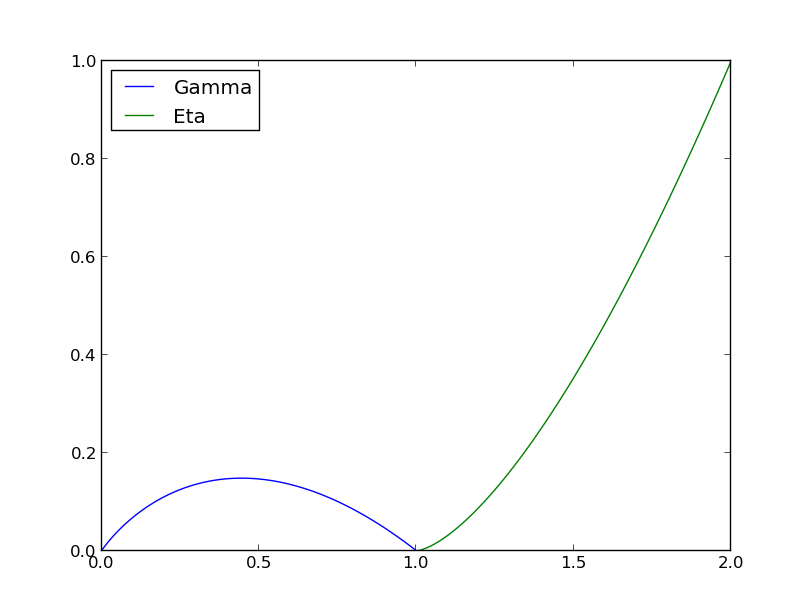
\includegraphics[width=0.9\linewidth]{./images/functions.png}}
            \caption{$\gamma$ and $\eta$}
    \end{figure}
 \begin{figure}[!htb]\centering
        \frame{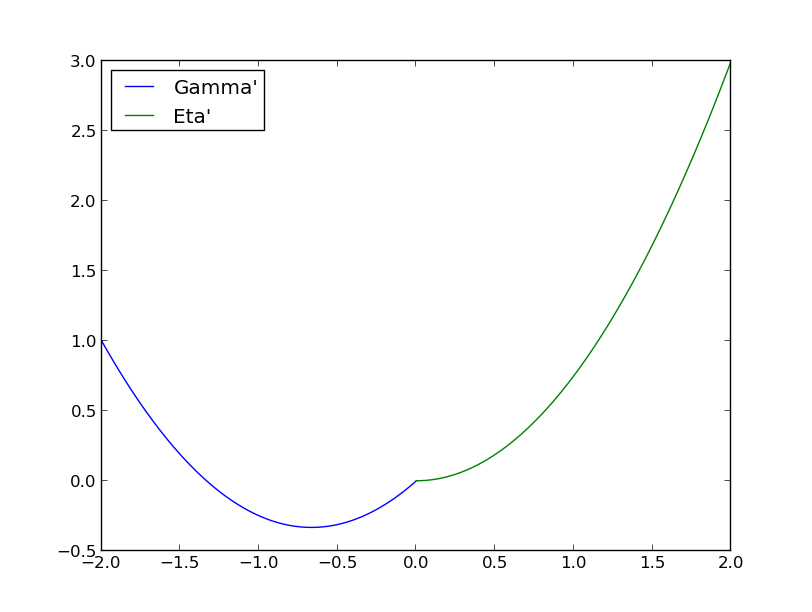
\includegraphics[width=0.9\linewidth]{./images/derivatives.png}}
        \caption{$\gamma'$ and $\eta'$}

    \end{figure}

\pagebreak

\subsection{NURBS: Non-uniform non-rational B-Splines}
\bigskip

\subsubsection{Problem statement}
\bigskip

Let $t_0=0, t_1=1, t_2=3, t_3=4, t_4=5$. Using these values, compute $B_{0,4}$ and each of the functions used in its definition. Then plot these functions on the interval $-3 \leq t \leq 8$.

\subsubsection{Answer}
\bigskip

We know that:
\begin{equation}
\left.\begin{aligned}
B_{i, 1} &=
\begin{cases}
   1 & \text{, } t_i \leq t \leq t_{i+1} \\
   0 & \text{, otherwise}
  \end{cases}& \\
B_{i,2}(t) &= \frac{t-t_i}{t_{i+1}-t_i}B_{i,1}(t) + \frac{t_{i+2}-t}{t_{i+2}-t_{i+1}}B_{i+1,1}(t)& \\
B_{i,3}(t) &= \frac{t-t_i}{t_{i+2}-t_i}B_{i,2}(t) + \frac{t_{i+3}-t}{t_{i+3}-t_{i+1}}B_{i+1,2}(t)& \\
B_{i,4}(t) &= \frac{t-t_i}{t_{i+3}-t_i}B_{i,3}(t) + \frac{t_{i+4}-t}{t_{i+4}-t_{i+1}}B_{i+1,3}(t)&\\\\
\end{aligned}\right.
\end{equation}

\noindent
For $i = 0$:
\begin{equation}
\left.\begin{aligned}
B_{0, 1}(t) &=
\begin{cases}
   1 & \text{, } t_0 \leq t \leq t_1 \\
   0 & \text{, otherwise}
  \end{cases}& \\
B_{0,2}(t) &= \frac{t-t_0}{t_1-t_0}B_{0,1}(t) + \frac{t_2-t}{t_2-t_1}B_{1,1}(t)& \\
B_{0,3}(t) &= \frac{t-t_0}{t_2-t_0}B_{0,2}(t) + \frac{t_3-t}{t_3-t_1}B_{1,2}(t)& \\
B_{0,4}(t) &= \frac{t-t_0}{t_3-t_0}B_{0,3}(t) + \frac{t_4-t}{t_4-t_1}B_{1,3}(t)&\\
B_{1,1}(t) &= \begin{cases}
   1 & \text{, } t_1 \leq t \leq t_2 \\
   0 & \text{, otherwise}
  \end{cases}&\\
B_{1,2}(t) &= \frac{t-t_1}{t_2-t_1}B_{1,1}(t) + \frac{t_3-t}{t_3-t_2}B_{2,1}(t)& \\
B_{1,3}(t) &= \frac{t-t_1}{t_3-t_1}B_{1,2}(t) + \frac{t_4-t}{t_4-t_2}B_{2,2}(t)& \\
B_{2,1}(t) &= \begin{cases}
   1 & \text{, } t_2 \leq t \leq t_3 \\
   0 & \text{, otherwise}
  \end{cases}&\\
B_{2,2}(t) &= \frac{t-t_2}{t_3-t_2}B_{2,1}(t) + \frac{t_4-t}{t_4-t_3}B_{3,1}(t)& \\
B_{3,1}(t) &= \begin{cases}
   1 & \text{, } t_3 \leq t \leq t_4 \\
   0 & \text{, otherwise}
  \end{cases}&\\\\
\end{aligned}\right.
\end{equation}

\noindent
Which gives us:
\begin{equation}
\left.\begin{aligned}
B_{0, 1}(t) &=
\begin{cases}
   1 & \text{, } 0 \leq t \leq 1 \\
   0 & \text{, otherwise}
  \end{cases}& \\
B_{0,2}(t) &= tB_{0,1}(t) + \frac{3-t}{2}B_{1,1}(t)& \\
B_{0,3}(t) &= \frac{t}{3}B_{0,2}(t) + \frac{4-t}{3}B_{1,2}(t)& \\
B_{0,4}(t) &= \frac{t}{4}B_{0,3}(t) + \frac{5-t}{4}B_{1,3}(t)&\\
B_{1,1}(t) &= \begin{cases}
   1 & \text{, } 1 \leq t \leq 3 \\
   0 & \text{, otherwise}
  \end{cases}&\\
    B_{1,2}(t) &= \frac{t-1}{2}B_{1,1}(t) + (4-t)B_{2,1}(t)& \\
B_{1,3}(t) &= \frac{t-1}{3}B_{1,2}(t) + \frac{5-t}{2}B_{2,2}(t)& \\
B_{2,1}(t) &= \begin{cases}
   1 & \text{, } 3 \leq t \leq 4 \\
   0 & \text{, otherwise}
  \end{cases}&\\
    B_{2,2}(t) &= (t-3)B_{2,1}(t) + (5-t)B_{3,1}(t)& \\
B_{3,1}(t) &= \begin{cases}
   1 & \text{, } 4 \leq t \leq 5 \\
   0 & \text{, otherwise}
  \end{cases}&\\\\
\end{aligned}\right.
\end{equation}


    \begin{figure}[!htb]\centering

            \frame{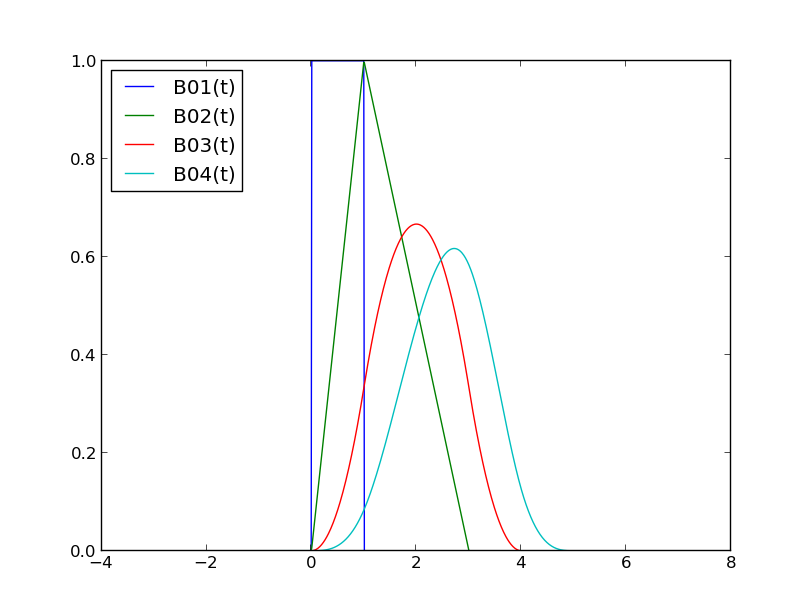
\includegraphics[width=0.9\linewidth]{./images/nurbs.png}}
            \caption{Plot of $B_{04}(t)$, $B_{03}(t)$, $B_{02}(t)$, $B_{01}(t)$}
    \end{figure}

\end{document}
